\documentclass[12pt]{report}
\usepackage[utf8]{inputenc}
\usepackage{amsmath,amsthm,amsfonts,amssymb,amscd}
\usepackage{multirow,booktabs}
\usepackage[table]{xcolor}
\usepackage{fullpage}
\usepackage{lastpage}
\usepackage{enumitem}
\usepackage{fancyhdr}
\usepackage{mathrsfs}
\usepackage{wrapfig}
\usepackage{setspace}
\usepackage{calc}
\usepackage{multicol}
\usepackage{cancel}
\usepackage[retainorgcmds]{IEEEtrantools}
\usepackage[margin=3cm]{geometry}
\usepackage{amsmath}
\newlength{\tabcont}
\setlength{\parindent}{0.0in}
\setlength{\parskip}{0.05in}
\usepackage{empheq}
\usepackage{framed}
\usepackage[most]{tcolorbox}
\usepackage{xcolor}
\colorlet{shadecolor}{orange!15}
\parindent 0in
\parskip 12pt
\geometry{margin=1in, headsep=0.25in}
\theoremstyle{definition}
\newtheorem{defn}{Definition}
\newtheorem{reg}{Rule}
\newtheorem{exer}{Exercise}
\newtheorem{note}{Note}

\usepackage[superscript,biblabel]{cite}
\usepackage{hyperref}
\hypersetup{colorlinks,linkcolor={blue},citecolor={blue},urlcolor={orange}}

\usepackage{graphicx}
% Path relative to the main .tex file
\graphicspath{ {./images/} }

\title{\textbf{Practical integrator using operational amplifier}}
\author{
  Russel Shawn Dsouza\\
  171EC143
  \and
  Sathvik S Prabhu\\
  171EC146
}
\date{}

\begin{document}
  \maketitle

  \section{Aim}
  To design and test a $\mu$A741-based voltage integrator for a sinusoidal input $V_{in}(t) = 2sin(4000\pi t)$.

  \section{Components required}

  \section{Theory}

  \section{Design}

  \section{Calculations}

  \section{Simulation}

  \section{Waveforms}

  \section{Observations}
  \begin{figure}
    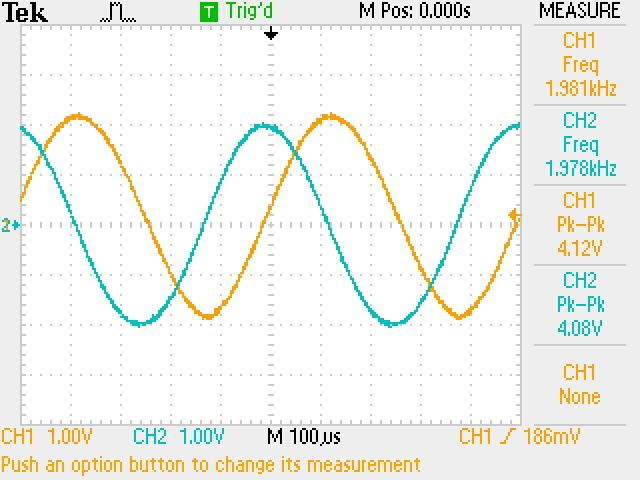
\includegraphics[width=\textwidth]{images/results_q1.jpeg}
    \caption{Result}
  \end{figure}

  \section{Result}

\end{document}
